\newpage
\section{File I/O}


% Introduzione
\subsection{Chiamata open}

I file I/O sono le \hl{funzioni che gestisce buffered I/O} ed in contrapposizione da quelle della libreria "stdlib". La chiamata open() fa parte di queste funzioni, i suoi argomenti sono:

\begin{itemize}
	\item \hl{arg}: path assoluto o relativo
	\item \hl{flag}: bit che indica l'\textbf{attivazione di alcune modalita'}. Si avrà allora a \textbf{settare il bit della flag a 1}:
	\item \hl{mode}: serve a dare i \textbf{privilegi con cui i file deve essere creato} (\textbf{da usare solo nella creazione del file})
\begin{lstlisting}
open(file, O_RDWR | O_APPEND | O_CREAT | O_TRUNC, file_mode)
\end{lstlisting}

		avremo allora $11000001010$ con:
		
		\begin{itemize}
			\item[] O\_RDWR = 2
			\item[] O\_APPEND = 8
			\item[] O\_CREAT = 512
			\item[] O\_TRUNC = 1024
		\end{itemize}
		
\end{itemize}


% Read e write flag
\subsection{Read e write flag}

I \hl{bit delle flag} abbiamo un modo "scomodo" per rappresentarle dato che non seguono la normale "accensione dei singoli bit":

\begin{lstlisting}
#define O_RDONLY   0x0000 /* reading only */
#define O_WRONLY   0x0001 /* writing only */
#define O_RDWR     0x0002 /* reading and writing */
#define O_ACCMODE  0x0003 /* above modes */
\end{lstlisting}

sono dette \hl{maschere} per leggere o scrivere.

Per quanto riguarda la chiamata read ci sono più casi in cui il numero di \hl{byte restituito e' minore di quello chiesto}:

\begin{enumerate}
	\item possiamo avere un valore di ritorno di 50 se chiedo di leggere 100 perché \textbf{ci sono solo 50 byte}
	\item quando legge da un \textbf{terminale}: la read ritorna quando dai invio
	\item quando legge da una \textbf{rete}: puoi leggere 100 byte ma se ne leggi 10 interrompe la lettura e ritorna, invece se non arriva nulla rimane in attesa
	\item quando legge da una \textbf{pipe}: se non arriva nulla rimane appesa, se arriva qualcosa interrompe e restituisce quello che ha letto
	\item quando \textbf{interrotta da un segnale} e alcuni dati sono stati letti gli restituisce
\end{enumerate} 


% Chiamata openat()
\subsection{Chiamata openat()}

\hl{Prende un file descriptor} (passato dalla open() sulla directory) di una directory per passare il path relativo a quella directory. La sua \hl{falla nel sistema} sta nella possibilità di \hl{continuare ad accedere a file anche dopo che sono cambiati i privilegi}, dato che lasciando aperta la sessione del file non saremo soggetti ai nuovi privilegi.

Questa chiamata è \hl{interessante per le Thread} che vogliono lavorare in un loro ambiente.


% Open flags
\subsection{Open flags}

Abbiamo un certo numero di \hl{flag standard} dichiarate dall'SUSv3, il resto possono essere a discrezione dei sistemi UNIX.

Le flags più usate sono:

\begin{itemize}
	\item \hl{O\_DIRECTORY}: \textbf{limita la chiamata} open ad una directory specifica

	\item \hl{O\_CREAT}: flag per dire che si vuole \textbf{creare un file}

	\item \hl{O\_TRUNC}: se vuoi creare un file nuovo ed ne esiste già uno, il \textbf{vecchio viene azzerato}

	\item \hl{O\_EXCL}: se il file già esiste fa \textbf{fallire la chiamata}
\end{itemize}


% Builtin umask
\subsection{Builtin umask}

È un \hl{valore presente in ogni processo} ed ereditato dal parent ma il child può comunque modificarla. Il valore restituito è un numero ottale (inizia con 0):

\begin{lstlisting}
$ umask
0022

$ ll file
-rw-r--r-- 1 docente staff 0 14 Ott 09:02 file
\end{lstlisting}

quindi la umask \hl{taglia i permessi dei file creati da quel processo}. Quindi, in questo caso, un 666 diventa 644.


% Chiamata lseek()
\subsection{Chiamata lseek()}

Per un file appena creato la sua "current position" si trova all'inizio del file, ci si \hl{potra' muovere nel file} tramite lseek(). Gli argomenti sono:

\begin{enumerate}
	\item \hl{file descriptor}
	
	\item \hl{offset}: per dire \textbf{dove ci si vuole spostare}
	
	\item \hl{whence}: indica \textbf{da quale punto} si deve applicare l'offset:
	
		\begin{itemize}
			\item SEEK\_SET: valore preciso da dove partire
			
			\item SEEK\_CUR: presa la current position inserire un \textbf{gap e poi scrivere} (può essere negativo)
			
			\item SEEK\_END: gap dal quale inserire \textbf{rispetto alla fine} del file. Se negativo scrivo prima, se positivo posso lasciare un \textbf{buco di byte} e poi scrivere. Nei nuovi sistemi i blocchi vuoti vengono allocati.
		\end{itemize}
	
	
\end{enumerate}

Un esempio di buco in un file dato da un numero positivo con SEEK\_END:

\begin{lstlisting}
#include "apue.h"
#include <fcntl.h>

char	buf1[] = "abcdefgh";
char	buf2[] = "ABCDEFGH";

int
main(void)
{
	int		fd;

	if ((fd = creat("file.hole", FILE_MODE)) < 0)
		err_sys("creat error");

	if (write(fd, buf1, 10) != 10)
		err_sys("buf1 write error");
	/* offset now = 10 */

	if (lseek(fd, 16384, SEEK_SET) == -1)
		err_sys("lseek error");
	/* offset now = 16384 */

	if (write(fd, buf2, 10) != 10)
		err_sys("buf2 write error");
	/* offset now = 16394 */

	exit(0);
}	
\end{lstlisting}

avremo:

\begin{lstlisting}
$ xxd file.hole
00000000: 6162 6364 6566 0000    abcdefgh........
00000010: 0000 0000 0000 0000    ................
00000020: 0000 0000 0000 0000    ................
00000030: 0000 0000 0000 0000    ................
00000040: 0000 0000 0000 0000    ................
00000050: 0000 0000 0000 0000    ................
00000060: 0000 0000 0000 0000    ................
00000070: 4142 4344 4546 4748    ABCDEFGH........
\end{lstlisting}

abbiamo che la memoria sul disco è:

\begin{lstlisting}
$ du -h file.hole 
1.6M	file.hole
\end{lstlisting}

invece la size del file è:

\begin{lstlisting}
$ stat -x file.hole 
  File: "file.hole"
  Size: 1638410      FileType: Regular File
  Mode: (0644/-rw-r--r--)         Uid: (  501/    matt)  Gid: (   20/   staff)
Device: 1,16   Inode: 27657406    Links: 1
Access: Fri Oct 14 09:59:17 2022
Modify: Fri Oct 14 09:57:59 2022
Change: Fri Oct 14 09:57:59 2022
 Birth: Fri Oct 14 09:47:24 2022
\end{lstlisting}

Possiamo avere dei \hl{file descriptor seekble} se il file è regolare o meno:

\begin{lstlisting}
#include "apue.h"

int
main(void)
{
	if (lseek(STDIN_FILENO, 0, SEEK_CUR) == -1)
		printf("cannot seek\n");
	else
		printf("seek OK\n");
	exit(0);
}
\end{lstlisting}


% I/O efficiency
\subsection{I/O efficiency}

Se devo \hl{trasferire una grande quantita' di dati} avrò una dimensione ottimale con la quale posso \hl{ottimizzare il passaggio dei blocchi di dati}. I tempi possono essere misurati con "time" per capire in che modo il nostro GB debba essere sezionato (in K, M, ...).

(provare a fare ciò tramite intro/mycat e tramite time capire le tempistiche (A CASA))

\begin{figure}[H]
\centering
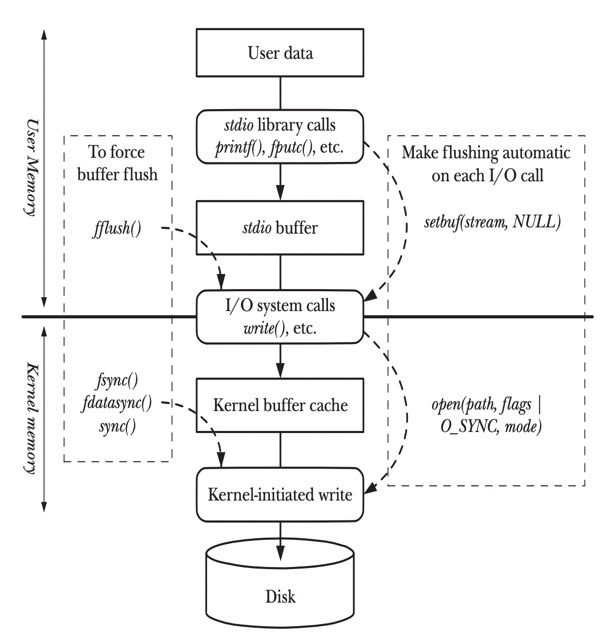
\includegraphics[scale=0.4]{unbuffio.jpeg}
\caption{Schema unbuffered I/O} 
\label{unbuffio}
\end{figure}


% File sharing
\subsection{File sharing}

Quando \hl{un processo accede ad un file} per utilizzarlo accade che:


\begin{figure}[H]
\centering
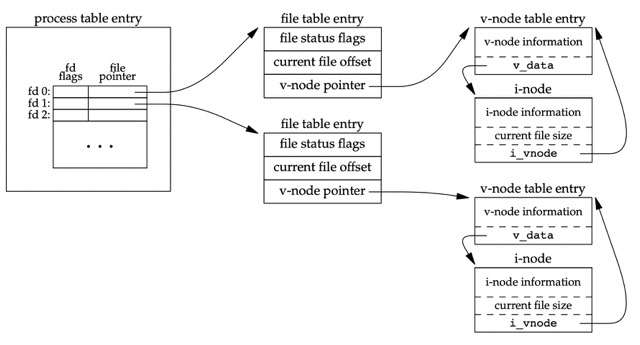
\includegraphics[scale=0.4]{1proc.jpeg}
\caption{Unico processo accede a un file} 
\label{1proc}
\end{figure}


Il processo è rappresentato dal "\hl{process table entry}" con i vari file descriptor con la loro flag e puntatore alla memoria delle \hl{file table entry}. Ogni \hl{file descriptor avra' una file table entry}, quindi ci saranno tanti file table quanti fd ci sono, con i seguenti dati:

\begin{itemize}
	\item \textbf{file status flags}: 
	\item \textbf{current file offset}: 
	\item \textbf{v-node pointer}: (con v=virtual) puntatore ad una v-node table entry che contiene i dati, cioè:
		\begin{itemize}
			\item \textbf{v-node information}
			\item \textbf{v\_data}: puntatore all'inode
		\end{itemize}
\end{itemize}


Potrebbe capitare che \hl{piu' processi si contengano un file} tra di loro per poterci accedere.


\begin{figure}[H]
\centering
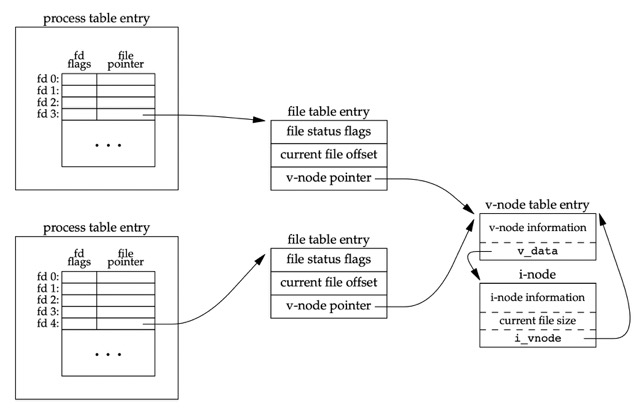
\includegraphics[scale=0.4]{2proc.jpeg}
\caption{Più processi accedono a file} 
\label{2proc}
\end{figure}


Ogni processo arriverà al file tramite 2 file table diverse ma con un \hl{"v-node prointer" allo stesso file}. Dato che 2 processi stanno contemporaneamente scrivendo servirà chi gestisce il tutto altrimenti ci sarà una \hl{sovrascrittura} dell'ultimo processo sugli altri.

In queste situazioni \hl{il kernel si intromette} per evitare di far "intromettere" altri processi durante l'esecuzione delle system call. Questo è possibile grazie alle \hl{operazioni atomiche} (tutto gestito dal programmatore del kernel). Un'esempio di operazioni atomiche è l'inserimento della \hl{flag O\_APPEND}.

Le \hl{chiamate per creare operazioni atomiche} con più system call sono:

\begin{itemize}
	\item \hl{pread()}: è come chiamare lseek() e dopo read()
	\item \hl{pwrite()}: come write() ma con un parametro offset che permette di effettuare un'operazione atomica scrivendo in un punto del file \textbf{senza rischio che le operazione di lseek e write si diano fastidio}. Vanno allora a fare più operazioni in una unica ma atomica
\end{itemize}


Un'altro flag da tenere sott'occhio è \hl{O\_EXCL}, in questo caso se il file da creare esite non viene creato. Potrebbe succedere che se il file non esiste e viene \hl{dato l'OK per crearlo} ma nel frattempo viene creato da un altro processo, allora \hl{il primo andra' a sovrascrivere}.

Quest'operazione viene usata per poter \hl{usare in modo esclusivo} il nome di un file da un processo in modo da non farlo utilizzare da un altro mentre lui esegue le sue operazioni su altri file (il file provvisorio verrà poi eliminato).


% dup & dup2
\subsection{dup \& dup2}

Vediamo le seguenti funzioni:

\begin{itemize}
	\item \hl{dup}: \textbf{prende un fd e restituisce un duplicato del fd}. Quindi \textbf{abbiamo 2 fd che puntano alla stessa file table}.

	\begin{figure}[H]
	\centering
	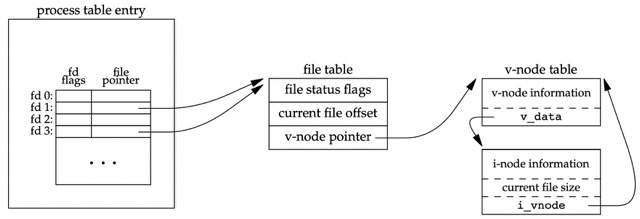
\includegraphics[scale=0.4]{dup.jpeg}
	\caption{dup function} 
	\label{dup}
	\end{figure}


	\item \hl{dup2}: prende un fd da duplicare \textbf{dicendogli anche il numero del fd}, se il numero che gli passiamo è già preso allora si \textbf{forza la chiusura} del fd e lo si assegna a ciò che vogliamo

\end{itemize}


Con le \hl{fork} avremo:


\begin{figure}[H]
\centering
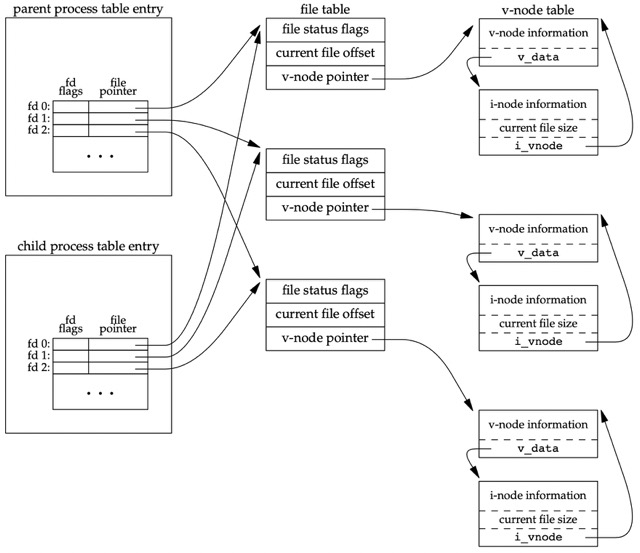
\includegraphics[scale=0.4]{forkproc.jpeg}
\caption{Fork con process table entry} 
\label{forkproc}
\end{figure}


dopo una fork i processi child e parent sono uno la copia dell'altro quindi avremo che i \hl{fd del child punteranno alle stesse file table} e quindi agli stessi spazi di memoria alla quale \hl{accedono entrambi}. Abbiamo quindi il problema che se il child modifica qualcosa lo vedrà anche il parent.


% Ridirezione ad un file
\subsection{Ridirezione ad un file}

Quindi apriamo un file ci viene dato un fd con numero minore (in genere 3), se faccio una \hl{dup2(3, 1)} abbiamo la ridirezione a file. \hl{A fare tutte le operazioni e' lo shell} e grazie alla eredità dei fd i processi child avranno già tutti i dati.

La gestire di queste operazioni dipende dal flag \hl{CLOEXEC}. Infatti quando lo shell vede la ridirezione ($>$) allora:

\begin{itemize}
	\item se sei il child esegui l'apertura del file
	\item ottiene fd 3
	\item esegui dup(3, 1)
	\item esegui una exec
	\item se il \hl{flag e' 0} (cioè non chiudere quando fai un exec) allora il child avrà in input l'output del parent
	\item se il \hl{flag e' 1} vogliamo che il file venga chiuso ed il fd riassegnato
\end{itemize}


% Funzione fcntl()
\subsection{Funzione fcntl()}

È un \hl{coltellino svizzero per controlli sul fd} e ha come parametri: 

\begin{itemize}
	\item fd
	\item \hl{cmd}: usato per \textbf{chiamare delle funzionalità} specifiche tramite flags:

		\begin{itemize}
			\item \textbf{F\_DUPFD}: si \textbf{duplica il fd} e tramite il terzo argomento avremo all'\textbf{assegnazione di un fd $\geq$ del valore di quell'argomento}
			\item \textbf{F\_GETFD, F\_SETFD}: get/set fd flag
			\item \textbf{F\_GETFL, F\_SETFL}: get/set file status flag (per cambiare il flag \textbf{mentre il file è ancora aperto})
			\item \textbf{F\_GETLK, F\_SETLK}: get/set record locks: servono a \textbf{bloccare parti di file}
		\end{itemize}
	
	\item "args"
\end{itemize}

Grazie al file fileflags.c possiamo vedere come è stato aperto il file:

\begin{lstlisting}
#include "apue.h"
#include <fcntl.h>

int
main(int argc, char *argv[])
{
	int		val;

	if (argc != 2)
		\

	if ((val = fcntl(atoi(argv[1]), F_GETFL, 0)) < 0)
		err_sys("fcntl error for fd %d", atoi(argv[1]));

	switch (val & O_ACCMODE) {
	case O_RDONLY:
		printf("read only");
		break;

	case O_WRONLY:
		printf("write only");
		break;

	case O_RDWR:
		printf("read write");
		break;

	default:
		err_dump("unknown access mode");
	}

	if (val & O_APPEND)
		printf(", append");
	if (val & O_NONBLOCK)
		printf(", nonblocking");
	if (val & O_SYNC)
		printf(", synchronous writes");

#if !defined(_POSIX_C_SOURCE) && defined(O_FSYNC) && (O_FSYNC != O_SYNC)
	if (val & O_FSYNC)
		printf(", synchronous writes");
#endif

	putchar('\n');
	exit(0);
}	
\end{lstlisting}

infatti abbiamo:

\begin{lstlisting}
$ ./fileflags 0 < /dev/ttys000
read only

$ ./fileflags 1 > prova.txt
$ cat prova.txt 
write only

$ ./fileflags 2 2>>prova.txt 
write only, append

$ ./fileflags 5 5<>prova.txt 
read write
\end{lstlisting}

per inserire o togliere i flag usiamo:

\begin{lstlisting}
val |= flags;		/* turn on flags */
val &= ~flag;		/* turn off flags */
\end{lstlisting}
